\documentclass[aspectratio=169]{beamer}

% ============================================
% PACKAGES
% ============================================
\usepackage{tikz}
\usetikzlibrary{positioning}
\usepackage{graphicx}
\usepackage{hyperref}
\usepackage{xcolor}
\usepackage{fancyhdr}
\usepackage{fontspec}
\usepackage{amsmath}
\usepackage{booktabs}
\usepackage{array}
\usepackage{colortbl}
\usepackage{listings}

% ============================================
% DATABRICKS COLOR PALETTE
% ============================================
\definecolor{databricksBlue}{RGB}{41, 49, 66}
\definecolor{databricksRed}{RGB}{220, 53, 69}
\definecolor{databricksYellow}{RGB}{255, 193, 7}
\definecolor{databricksGreen}{RGB}{76, 175, 80}
\definecolor{databricksGray}{RGB}{128, 128, 128}
\definecolor{databricksLightGray}{RGB}{245, 245, 245}
\definecolor{databricksWhite}{RGB}{255, 255, 255}

% ============================================
% BEAMER THEME CONFIGURATION
% ============================================
\usetheme{default}
\usecolortheme{default}

% Set background and text colors
\setbeamercolor{background canvas}{bg=databricksWhite}
\setbeamercolor{normal text}{fg=databricksBlue}
\setbeamercolor{frametitle}{fg=databricksWhite, bg=databricksBlue}
\setbeamercolor{title}{fg=databricksWhite}
\setbeamercolor{subtitle}{fg=databricksLightGray}
\setbeamercolor{author}{fg=databricksWhite}
\setbeamercolor{date}{fg=databricksLightGray}
\setbeamercolor{institute}{fg=databricksLightGray}

% Item colors
\setbeamercolor{itemize item}{fg=databricksBlue}
\setbeamercolor{itemize subitem}{fg=databricksRed}
\setbeamercolor{itemize subsubitem}{fg=databricksGreen}

% Block colors
\setbeamercolor{block title}{fg=databricksWhite, bg=databricksBlue}
\setbeamercolor{block body}{fg=databricksBlue, bg=databricksLightGray}

% Item symbols
\setbeamertemplate{itemize item}{\textcolor{databricksBlue}{$\bullet$}}
\setbeamertemplate{itemize subitem}{\textcolor{databricksRed}{$\triangleright$}}
\setbeamertemplate{itemize subsubitem}{\textcolor{databricksGreen}{$\diamond$}}

% Remove navigation symbols
\setbeamertemplate{navigation symbols}{}

% ============================================
% CUSTOM TITLE PAGE
% ============================================
\defbeamertemplate*{title page}{customized}[1][]
{
  \begin{tikzpicture}[remember picture, overlay]
    \fill[databricksBlue] (current page.north west) rectangle (current page.south east);
    
    % Subtitle (above title)
    \node[anchor=center, text=databricksLightGray, font=\large, text width=12cm, align=center] 
      at ([yshift=1.5cm]current page.center) {\insertsubtitle};
    
    % Title
    \node[anchor=center, text=databricksWhite, font=\Huge\bfseries, text width=14cm, align=center] 
      at ([yshift=0.3cm]current page.center) {\inserttitle};
    
    % Decorative accent line
    \draw[databricksRed, line width=3pt] ([yshift=-0.5cm, xshift=-5cm]current page.center) -- ([yshift=-0.5cm, xshift=5cm]current page.center);
    
    % Author
    \node[anchor=center, text=databricksYellow, font=\normalsize] 
      at ([yshift=-1.3cm]current page.center) {\insertauthor};
    
    % Date
    \node[anchor=center, text=databricksLightGray, font=\small] 
      at ([yshift=-2.1cm]current page.center) {\insertdate};
  \end{tikzpicture}
}

% ============================================
% CUSTOM FRAME TITLE
% ============================================
\setbeamertemplate{frametitle}{
  \begin{beamercolorbox}[wd=\paperwidth, ht=1.2cm, dp=0.3cm]{frametitle}
    \hspace{0.5cm}\usebeamerfont{frametitle}\insertframetitle
  \end{beamercolorbox}
}

% ============================================
% CUSTOM FOOTER
% ============================================
\setbeamertemplate{footline}{
  \begin{tikzpicture}[remember picture, overlay]
    \fill[databricksBlue] (current page.south west) rectangle ([yshift=0.6cm]current page.south east);
    
    % Left: Easy AI Labs
    \node[anchor=west, text=databricksWhite, font=\tiny] 
      at ([xshift=0.5cm, yshift=0.3cm]current page.south west) 
      {\href{https://easy-ai-labs.lovable.app/}{\textcolor{databricksWhite}{Easy AI Labs}}};
    
    % Center: Yash Kavaiya
    \node[anchor=center, text=databricksWhite, font=\tiny] 
      at ([yshift=0.3cm]current page.south) 
      {\href{https://www.linkedin.com/in/yashkavaiya}{\textcolor{databricksWhite}{Yash Kavaiya}}};
    
    % Right: Gen AI Guru
    \node[anchor=east, text=databricksWhite, font=\tiny] 
      at ([xshift=-1.5cm, yshift=0.3cm]current page.south east) 
      {\href{https://www.linkedin.com/company/genai-guru}{\textcolor{databricksWhite}{Gen AI Guru}}};
    
    % Slide counter
    \node[anchor=east, text=databricksYellow, font=\tiny\bfseries] 
      at ([xshift=-0.3cm, yshift=0.3cm]current page.south east) 
      {\insertframenumber/\inserttotalframenumber};
  \end{tikzpicture}
}

% ============================================
% CODE LISTING STYLE
% ============================================
\lstset{
  basicstyle=\ttfamily\scriptsize,
  backgroundcolor=\color{databricksLightGray},
  keywordstyle=\color{databricksBlue}\bfseries,
  stringstyle=\color{databricksGreen},
  commentstyle=\color{databricksGray}\itshape,
  breaklines=true,
  frame=single,
  rulecolor=\color{databricksBlue},
  showstringspaces=false
}

% ============================================
% DOCUMENT INFO
% ============================================
\title{Performance Optimization}
\subtitle{Delta Lake \& Spark | Day 10}
\author{Databricks 14-Days AI Challenge}
\date{January 2026}

% ============================================
% DOCUMENT CONTENT
% ============================================
\begin{document}

% Title Slide
\frame{\titlepage}

% ============================================
% TABLE OF CONTENTS
% ============================================
\begin{frame}{Agenda}
  \begin{columns}[T]
    \begin{column}{0.5\textwidth}
      \begin{itemize}
        \item \textcolor{databricksBlue}{\textbf{Introduction to Performance Optimization}}
        \item \textcolor{databricksBlue}{\textbf{Query Execution Plans}}
        \item \textcolor{databricksBlue}{\textbf{Partitioning Strategies}}
      \end{itemize}
    \end{column}
    \begin{column}{0.5\textwidth}
      \begin{itemize}
        \item \textcolor{databricksBlue}{\textbf{OPTIMIZE \& ZORDER}}
        \item \textcolor{databricksBlue}{\textbf{Caching Techniques}}
        \item \textcolor{databricksBlue}{\textbf{Best Practices}}
      \end{itemize}
    \end{column}
  \end{columns}
\end{frame}

% ============================================
% INTRODUCTION
% ============================================
\begin{frame}{Why Performance Optimization Matters}
  \begin{columns}[T]
    \begin{column}{0.55\textwidth}
      \textcolor{databricksBlue}{\textbf{The Library Analogy:}}
      \begin{itemize}
        \item Scattered books = slow searches
        \item Organized by genre/author = fast lookups
      \end{itemize}
      \vspace{0.3cm}
      \textcolor{databricksRed}{\textbf{Key Benefits:}}
      \begin{itemize}
        \item Reduces compute costs
        \item Improves user experience
        \item Enables larger dataset processing
        \item Reduces resource contention
      \end{itemize}
    \end{column}
    \begin{column}{0.45\textwidth}
      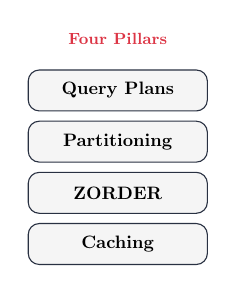
\begin{tikzpicture}[scale=0.65, transform shape]
        \node[draw=databricksBlue, fill=databricksLightGray, rounded corners, minimum width=3.5cm, minimum height=0.8cm] (qp) at (0,3) {\textbf{Query Plans}};
        \node[draw=databricksBlue, fill=databricksLightGray, rounded corners, minimum width=3.5cm, minimum height=0.8cm] (pt) at (0,2) {\textbf{Partitioning}};
        \node[draw=databricksBlue, fill=databricksLightGray, rounded corners, minimum width=3.5cm, minimum height=0.8cm] (zo) at (0,1) {\textbf{ZORDER}};
        \node[draw=databricksBlue, fill=databricksLightGray, rounded corners, minimum width=3.5cm, minimum height=0.8cm] (ca) at (0,0) {\textbf{Caching}};
        \node[font=\small\bfseries, text=databricksRed] at (0,4) {Four Pillars};
      \end{tikzpicture}
    \end{column}
  \end{columns}
\end{frame}

% ============================================
% FOUR PILLARS TABLE
% ============================================
\begin{frame}{The Four Pillars of Optimization}
  \centering
  \begin{tabular}{>{\columncolor{databricksLightGray}}l p{5cm} p{5cm}}
    \toprule
    \rowcolor{databricksBlue}
    \textcolor{databricksWhite}{\textbf{Pillar}} & \textcolor{databricksWhite}{\textbf{What It Does}} & \textcolor{databricksWhite}{\textbf{When to Use}} \\
    \midrule
    \textbf{Query Plans} & Shows HOW Spark executes your query & Debugging slow queries \\
    \midrule
    \textbf{Partitioning} & Physically organizes data on disk & Large tables with filter patterns \\
    \midrule
    \textbf{ZORDER} & Optimizes data layout within files & Multi-column filter queries \\
    \midrule
    \textbf{Caching} & Keeps data in memory & Repeated access to same data \\
    \bottomrule
  \end{tabular}
\end{frame}

% ============================================
% QUERY EXECUTION PLANS
% ============================================
\begin{frame}{Query Execution Plans}
  \textcolor{databricksBlue}{\textbf{A "Recipe" for Your Data:}} Shows every step Spark takes to transform your query into results.
  
  \vspace{0.3cm}
  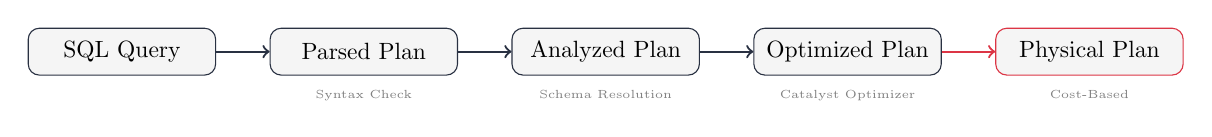
\begin{tikzpicture}[node distance=0.8cm, scale=0.85, transform shape]
    \node[draw=databricksBlue, fill=databricksLightGray, rounded corners, minimum width=2.8cm, minimum height=0.7cm] (a) {SQL Query};
    \node[draw=databricksBlue, fill=databricksLightGray, rounded corners, minimum width=2.8cm, minimum height=0.7cm, right=of a] (b) {Parsed Plan};
    \node[draw=databricksBlue, fill=databricksLightGray, rounded corners, minimum width=2.8cm, minimum height=0.7cm, right=of b] (c) {Analyzed Plan};
    \node[draw=databricksBlue, fill=databricksLightGray, rounded corners, minimum width=2.8cm, minimum height=0.7cm, right=of c] (d) {Optimized Plan};
    \node[draw=databricksRed, fill=databricksLightGray, rounded corners, minimum width=2.8cm, minimum height=0.7cm, right=of d] (e) {Physical Plan};
    
    \draw[->, thick, databricksBlue] (a) -- (b);
    \draw[->, thick, databricksBlue] (b) -- (c);
    \draw[->, thick, databricksBlue] (c) -- (d);
    \draw[->, thick, databricksRed] (d) -- (e);
    
    \node[font=\tiny, text=databricksGray, below=0.1cm of b] {Syntax Check};
    \node[font=\tiny, text=databricksGray, below=0.1cm of c] {Schema Resolution};
    \node[font=\tiny, text=databricksGray, below=0.1cm of d] {Catalyst Optimizer};
    \node[font=\tiny, text=databricksGray, below=0.1cm of e] {Cost-Based};
  \end{tikzpicture}
\end{frame}

% ============================================
% FOUR PHASES DETAIL
% ============================================
\begin{frame}{The Four Phases of Query Planning}
  \begin{columns}[T]
    \begin{column}{0.5\textwidth}
      \textcolor{databricksBlue}{\textbf{Phase 1: Parsed Logical Plan}}
      \begin{itemize}
        \item Parses SQL into abstract syntax tree
        \item Checks for syntax errors
        \item No validation against tables yet
      \end{itemize}
      
      \vspace{0.2cm}
      \textcolor{databricksBlue}{\textbf{Phase 2: Analyzed Logical Plan}}
      \begin{itemize}
        \item Validates table/column names
        \item Resolves data types
        \item Checks permissions
      \end{itemize}
    \end{column}
    \begin{column}{0.5\textwidth}
      \textcolor{databricksRed}{\textbf{Phase 3: Optimized Logical Plan}}
      \begin{itemize}
        \item Catalyst optimizer rules
        \item Predicate pushdown
        \item Projection pruning
      \end{itemize}
      
      \vspace{0.2cm}
      \textcolor{databricksGreen}{\textbf{Phase 4: Physical Plan}}
      \begin{itemize}
        \item Converts to physical operations
        \item Chooses join strategies
        \item Determines data exchange
      \end{itemize}
    \end{column}
  \end{columns}
\end{frame}

% ============================================
% EXPLAIN OUTPUT
% ============================================
\begin{frame}[fragile]{Understanding explain(True) Output}
\begin{lstlisting}[language=Python, basicstyle=\ttfamily\tiny]
spark.sql("SELECT * FROM silver.events WHERE event_type='purchase'").explain(True)
\end{lstlisting}
  
  \vspace{0.2cm}
  \begin{columns}[T]
    \begin{column}{0.5\textwidth}
      \textcolor{databricksBlue}{\textbf{Sample Output:}}
\begin{lstlisting}[basicstyle=\ttfamily\tiny, language=SQL]
== Physical Plan ==
*(1) Filter (event_type = purchase)
+- *(1) ColumnarToRow
   +- FileScan parquet
      PushedFilters: [EqualTo(event_type,purchase)]
\end{lstlisting}
    \end{column}
    \begin{column}{0.5\textwidth}
      \textcolor{databricksRed}{\textbf{Key Indicators:}}
      \begin{itemize}
        \item \texttt{*(1)} = Whole-stage codegen \textcolor{databricksGreen}{(good!)}
        \item \texttt{PushedFilters} = Filter optimized
        \item \texttt{PartitionFilters} = Partition pruning
      \end{itemize}
    \end{column}
  \end{columns}
\end{frame}

% ============================================
% PHYSICAL PLAN TERMS
% ============================================
\begin{frame}{Key Terms in Physical Plans}
  \centering
  \footnotesize
  \begin{tabular}{>{\columncolor{databricksLightGray}}l l l}
    \toprule
    \rowcolor{databricksBlue}
    \textcolor{databricksWhite}{\textbf{Term}} & \textcolor{databricksWhite}{\textbf{Meaning}} & \textcolor{databricksWhite}{\textbf{Performance Impact}} \\
    \midrule
    FileScan & Reading from disk & Base cost \\
    Filter & Removing rows & \textcolor{databricksGreen}{Good if pushed to scan} \\
    Project & Selecting columns & \textcolor{databricksGreen}{Good if reduces data} \\
    \rowcolor{databricksLightGray}
    Exchange & Shuffle between nodes & \textcolor{databricksRed}{Expensive!} \\
    BroadcastExchange & Small table broadcast & \textcolor{databricksGreen}{Efficient for joins} \\
    SortMergeJoin & Both sides sorted & Moderate cost \\
    BroadcastHashJoin & One side broadcast & \textcolor{databricksGreen}{Best for small tables} \\
    HashAggregate & Grouping operation & Memory intensive \\
    \bottomrule
  \end{tabular}
  
  \vspace{0.3cm}
  \textcolor{databricksRed}{\textbf{Red Flags:}} Multiple Exchanges | SortMergeJoin on small tables | No PushedFilters
\end{frame}

% ============================================
% PARTITIONING INTRO
% ============================================
\begin{frame}{What is Partitioning?}
  \begin{columns}[T]
    \begin{column}{0.55\textwidth}
      \textcolor{databricksBlue}{\textbf{Definition:}} Divides table into separate folders on disk based on column values.
      
      \vspace{0.3cm}
      \textcolor{databricksRed}{\textbf{Filing Cabinet Analogy:}}
      \begin{itemize}
        \item \textbf{Without:} All documents in one drawer
        \item \textbf{With:} Separate drawers for 2022, 2023, 2024
        \item Finding "2024 docs" = open only one drawer
      \end{itemize}
      
      \vspace{0.2cm}
      \textcolor{databricksGreen}{\textbf{Benefit:}} Spark reads only relevant folders instead of scanning everything.
    \end{column}
    \begin{column}{0.45\textwidth}
      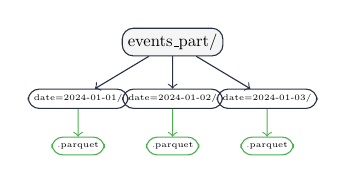
\begin{tikzpicture}[scale=0.6, transform shape]
        \node[draw=databricksBlue, fill=databricksLightGray, rounded corners] (root) at (0,0) {events\_part/};
        \node[draw=databricksBlue, rounded corners, font=\tiny] (d1) at (-2,-1.2) {date=2024-01-01/};
        \node[draw=databricksBlue, rounded corners, font=\tiny] (d2) at (0,-1.2) {date=2024-01-02/};
        \node[draw=databricksBlue, rounded corners, font=\tiny] (d3) at (2,-1.2) {date=2024-01-03/};
        \node[draw=databricksGreen, rounded corners, font=\tiny] (p1) at (-2,-2.2) {.parquet};
        \node[draw=databricksGreen, rounded corners, font=\tiny] (p2) at (0,-2.2) {.parquet};
        \node[draw=databricksGreen, rounded corners, font=\tiny] (p3) at (2,-2.2) {.parquet};
        
        \draw[->, databricksBlue] (root) -- (d1);
        \draw[->, databricksBlue] (root) -- (d2);
        \draw[->, databricksBlue] (root) -- (d3);
        \draw[->, databricksGreen] (d1) -- (p1);
        \draw[->, databricksGreen] (d2) -- (p2);
        \draw[->, databricksGreen] (d3) -- (p3);
      \end{tikzpicture}
    \end{column}
  \end{columns}
\end{frame}

% ============================================
% CREATING PARTITIONED TABLE
% ============================================
\begin{frame}[fragile]{Creating a Partitioned Table}
\begin{lstlisting}[language=SQL, basicstyle=\ttfamily\small]
CREATE TABLE silver.events_part
USING DELTA
PARTITIONED BY (event_date, event_type)
AS SELECT * FROM silver.events
\end{lstlisting}
  
  \vspace{0.3cm}
  \centering
  \footnotesize
  \begin{tabular}{>{\columncolor{databricksLightGray}}l p{8cm}}
    \toprule
    \rowcolor{databricksBlue}
    \textcolor{databricksWhite}{\textbf{Component}} & \textcolor{databricksWhite}{\textbf{Purpose}} \\
    \midrule
    \texttt{CREATE TABLE} & Creates new table in silver schema \\
    \texttt{USING DELTA} & Specifies Delta Lake format (ACID, time travel) \\
    \texttt{PARTITIONED BY} & Creates folder hierarchy: event\_date → event\_type \\
    \texttt{AS SELECT *} & Populates with data from source table \\
    \bottomrule
  \end{tabular}
\end{frame}

% ============================================
% PARTITION PRUNING
% ============================================
\begin{frame}[fragile]{Partition Pruning in Action}
\begin{lstlisting}[language=SQL, basicstyle=\ttfamily\small]
SELECT * FROM silver.events_part 
WHERE event_date = '2024-01-15' AND event_type = 'purchase'
\end{lstlisting}
  
  \vspace{0.3cm}
  \begin{columns}[T]
    \begin{column}{0.5\textwidth}
      \textcolor{databricksRed}{\textbf{Without Partition Pruning:}}
      \begin{itemize}
        \item Scans ALL data files
        \item Reads then filters
        \item \textcolor{databricksRed}{Slow and expensive}
      \end{itemize}
    \end{column}
    \begin{column}{0.5\textwidth}
      \textcolor{databricksGreen}{\textbf{With Partition Pruning:}}
      \begin{itemize}
        \item Reads ONLY matching folder
        \item Skips irrelevant partitions
        \item \textcolor{databricksGreen}{Fast and efficient}
      \end{itemize}
    \end{column}
  \end{columns}
  
  \vspace{0.3cm}
  \centering
  \textcolor{databricksBlue}{\textbf{Spark reads only:}} \texttt{events\_part/event\_date=2024-01-15/event\_type=purchase/}
\end{frame}

% ============================================
% CHOOSING PARTITION COLUMNS
% ============================================
\begin{frame}{Choosing Partition Columns}
  \begin{columns}[T]
    \begin{column}{0.5\textwidth}
      \textcolor{databricksGreen}{\textbf{Good Partition Columns:}}
      \begin{itemize}
        \item Low cardinality (10-1000 unique values)
        \item Frequently used in WHERE clauses
        \item Used in joins as keys
        \item Time-based (date, month, year)
      \end{itemize}
    \end{column}
    \begin{column}{0.5\textwidth}
      \textcolor{databricksRed}{\textbf{Bad Partition Columns:}}
      \begin{itemize}
        \item High cardinality (millions of values)
          \begin{itemize}
            \item Creates millions of tiny folders
          \end{itemize}
        \item Columns rarely filtered on
        \item Columns that change frequently
      \end{itemize}
    \end{column}
  \end{columns}
\end{frame}

% ============================================
% CARDINALITY GUIDELINES
% ============================================
\begin{frame}{Cardinality Guidelines}
  \centering
  \footnotesize
  \begin{tabular}{>{\columncolor{databricksLightGray}}l l l}
    \toprule
    \rowcolor{databricksBlue}
    \textcolor{databricksWhite}{\textbf{Cardinality}} & \textcolor{databricksWhite}{\textbf{Example}} & \textcolor{databricksWhite}{\textbf{Recommendation}} \\
    \midrule
    Very Low (<10) & status, region & \textcolor{databricksGreen}{Good for 2nd-level partition} \\
    Low (10-100) & country, event\_type & \textcolor{databricksGreen}{Good partition column} \\
    Medium (100-1000) & city, product\_category & \textcolor{databricksYellow}{Use with caution} \\
    High (1000-10000) & user\_segment & \textcolor{databricksRed}{Consider ZORDER instead} \\
    Very High (>10000) & user\_id, timestamp & \textcolor{databricksRed}{Never partition, use ZORDER} \\
    \bottomrule
  \end{tabular}
  
  \vspace{0.4cm}
  \textcolor{databricksBlue}{\textbf{Best Practice:}} Order partitions from lowest to highest cardinality
\end{frame}

% ============================================
% OPTIMIZE INTRO
% ============================================
\begin{frame}{The Small Files Problem}
  \begin{columns}[T]
    \begin{column}{0.5\textwidth}
      \textcolor{databricksBlue}{\textbf{Causes:}}
      \begin{itemize}
        \item Streaming micro-batches
        \item Frequent small updates
        \item Upsert operations
        \item Individual inserts
      \end{itemize}
    \end{column}
    \begin{column}{0.5\textwidth}
      \textcolor{databricksRed}{\textbf{Why It's Bad:}}
      \begin{itemize}
        \item Overhead per file (metadata ops)
        \item Inefficient reads
        \item Memory pressure on driver
        \item Slower query planning
      \end{itemize}
    \end{column}
  \end{columns}
  
  \vspace{0.3cm}
  \begin{center}
    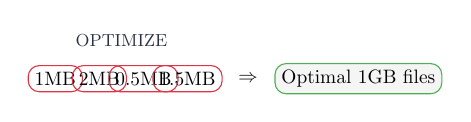
\begin{tikzpicture}[scale=0.7, transform shape]
      \node[draw=databricksRed, rounded corners, minimum width=0.5cm] at (0,0) {1MB};
      \node[draw=databricksRed, rounded corners, minimum width=0.5cm] at (0.8,0) {2MB};
      \node[draw=databricksRed, rounded corners, minimum width=0.5cm] at (1.6,0) {0.5MB};
      \node[draw=databricksRed, rounded corners, minimum width=0.5cm] at (2.4,0) {1.5MB};
      \node at (3.5,0) {$\Rightarrow$};
      \node[draw=databricksGreen, fill=databricksLightGray, rounded corners, minimum width=2cm] at (5.5,0) {Optimal 1GB files};
      \node[font=\small, text=databricksBlue] at (1.2,0.7) {OPTIMIZE};
    \end{tikzpicture}
  \end{center}
\end{frame}

% ============================================
% ZORDER EXPLANATION
% ============================================
\begin{frame}[fragile]{What is ZORDER?}
  \textcolor{databricksBlue}{\textbf{Definition:}} Co-locates related data within files using Z-order curve (Morton code).
  
  \vspace{0.2cm}
  \begin{columns}[T]
    \begin{column}{0.55\textwidth}
      \textcolor{databricksRed}{\textbf{Card Deck Analogy:}}
      \begin{itemize}
        \item Normal sort: All hearts, then diamonds
        \item ZORDER: Similar values across MULTIPLE attributes end up near each other
      \end{itemize}
      
      \vspace{0.2cm}
      \textcolor{databricksGreen}{\textbf{The Math:}}
      $$Z = \text{interleave}(x_{binary}, y_{binary})$$
    \end{column}
    \begin{column}{0.45\textwidth}
      \footnotesize
      \textcolor{databricksBlue}{\textbf{Z-order Pattern:}}
\begin{lstlisting}[basicstyle=\ttfamily\scriptsize]
y
3 |  5   7  13  15
2 |  4   6  12  14
1 |  1   3   9  11
0 |  0   2   8  10
  +---------------
     0   1   2   3  x
\end{lstlisting}
    \end{column}
  \end{columns}
\end{frame}

% ============================================
% ZORDER COMMAND
% ============================================
\begin{frame}[fragile]{OPTIMIZE with ZORDER}
\begin{lstlisting}[language=SQL, basicstyle=\ttfamily\small]
OPTIMIZE silver.events_part ZORDER BY (user_id, product_id)
\end{lstlisting}
  
  \vspace{0.3cm}
  \begin{columns}[T]
    \begin{column}{0.5\textwidth}
      \textcolor{databricksRed}{\textbf{Without ZORDER:}}
      \begin{itemize}
        \item user\_id scattered across ALL files
        \item Must scan everything
        \item \textcolor{databricksRed}{No data skipping}
      \end{itemize}
    \end{column}
    \begin{column}{0.5\textwidth}
      \textcolor{databricksGreen}{\textbf{With ZORDER:}}
      \begin{itemize}
        \item user\_id concentrated in FEW files
        \item Skip most files using min/max stats
        \item \textcolor{databricksGreen}{Efficient data skipping}
      \end{itemize}
    \end{column}
  \end{columns}
  
  \vspace{0.3cm}
  \textcolor{databricksBlue}{\textbf{Best Practice:}} Choose 2-4 most filtered columns; first column gets most benefit
\end{frame}

% ============================================
% CACHING INTRO
% ============================================
\begin{frame}{Caching Techniques}
  \textcolor{databricksBlue}{\textbf{Definition:}} Stores data in memory (RAM) for faster subsequent reads.
  
  \vspace{0.3cm}
  \centering
  \footnotesize
  \begin{tabular}{>{\columncolor{databricksLightGray}}l c p{5cm}}
    \toprule
    \rowcolor{databricksBlue}
    \textcolor{databricksWhite}{\textbf{Scenario}} & \textcolor{databricksWhite}{\textbf{Cache?}} & \textcolor{databricksWhite}{\textbf{Why}} \\
    \midrule
    Same DataFrame used 5+ times & \textcolor{databricksGreen}{\checkmark} & Avoids repeated computation \\
    Interactive data exploration & \textcolor{databricksGreen}{\checkmark} & Fast iterations \\
    ML training loops & \textcolor{databricksGreen}{\checkmark} & Features reread many times \\
    One-time transformation & \textcolor{databricksRed}{\texttimes} & Cache overhead not worth it \\
    Data larger than cluster memory & \textcolor{databricksRed}{\texttimes} & Causes spilling to disk \\
    \bottomrule
  \end{tabular}
\end{frame}

% ============================================
% CACHE VS PERSIST
% ============================================
\begin{frame}[fragile]{Cache vs Persist}
  \begin{columns}[T]
    \begin{column}{0.5\textwidth}
\begin{lstlisting}[language=Python, basicstyle=\ttfamily\small]
# Cache - memory only
df.cache()

# Persist - flexible
from pyspark import StorageLevel
df.persist(StorageLevel.MEMORY_AND_DISK)
\end{lstlisting}
    \end{column}
    \begin{column}{0.5\textwidth}
      \textcolor{databricksRed}{\textbf{Important:}} \texttt{.cache()} is \textbf{lazy}!
      
      \vspace{0.2cm}
      Data isn't cached until an action runs:
\begin{lstlisting}[language=Python, basicstyle=\ttfamily\small]
cached = spark.table("events").cache()
cached.count()  # Triggers caching
\end{lstlisting}
    \end{column}
  \end{columns}
  
  \vspace{0.3cm}
  \textcolor{databricksBlue}{\textbf{Release Cache:}} \texttt{cached.unpersist()} or \texttt{spark.catalog.clearCache()}
\end{frame}

% ============================================
% STORAGE LEVELS
% ============================================
\begin{frame}{Storage Levels}
  \centering
  \footnotesize
  \begin{tabular}{>{\columncolor{databricksLightGray}}l c c c c}
    \toprule
    \rowcolor{databricksBlue}
    \textcolor{databricksWhite}{\textbf{Level}} & \textcolor{databricksWhite}{\textbf{Memory}} & \textcolor{databricksWhite}{\textbf{Disk}} & \textcolor{databricksWhite}{\textbf{Serialized}} & \textcolor{databricksWhite}{\textbf{Replicated}} \\
    \midrule
    MEMORY\_ONLY & \textcolor{databricksGreen}{\checkmark} & \texttimes & \texttimes & \texttimes \\
    MEMORY\_AND\_DISK & \textcolor{databricksGreen}{\checkmark} & \textcolor{databricksGreen}{\checkmark} & \texttimes & \texttimes \\
    MEMORY\_ONLY\_SER & \textcolor{databricksGreen}{\checkmark} & \texttimes & \textcolor{databricksGreen}{\checkmark} & \texttimes \\
    MEMORY\_AND\_DISK\_SER & \textcolor{databricksGreen}{\checkmark} & \textcolor{databricksGreen}{\checkmark} & \textcolor{databricksGreen}{\checkmark} & \texttimes \\
    DISK\_ONLY & \texttimes & \textcolor{databricksGreen}{\checkmark} & \textcolor{databricksGreen}{\checkmark} & \texttimes \\
    MEMORY\_ONLY\_2 & \textcolor{databricksGreen}{\checkmark} & \texttimes & \texttimes & \textcolor{databricksGreen}{\checkmark} \\
    \bottomrule
  \end{tabular}
\end{frame}

% ============================================
% DELTA CACHE VS SPARK CACHE
% ============================================
\begin{frame}{Delta Cache vs Spark Cache}
  \centering
  \footnotesize
  \begin{tabular}{>{\columncolor{databricksLightGray}}l p{4.5cm} p{4.5cm}}
    \toprule
    \rowcolor{databricksBlue}
    \textcolor{databricksWhite}{\textbf{Feature}} & \textcolor{databricksWhite}{\textbf{Spark Cache}} & \textcolor{databricksWhite}{\textbf{Delta Cache}} \\
    \midrule
    Location & Executor memory & Local SSD \\
    Survives Restart & No & Yes \\
    Format & Deserialized objects & Compressed Parquet \\
    Best For & Repeated DataFrame ops & Repeated file reads \\
    Management & Manual (.cache/.unpersist) & Automatic \\
    \bottomrule
  \end{tabular}
\end{frame}

% ============================================
% OPTIMIZATION DECISION TREE
% ============================================
\begin{frame}{Optimization Decision Tree}
  \centering
  \begin{tikzpicture}[scale=0.55, transform shape, 
    node distance=0.8cm,
    decision/.style={diamond, draw=databricksBlue, fill=databricksLightGray, text width=1.8cm, align=center, inner sep=1pt},
    action/.style={rectangle, draw=databricksGreen, fill=databricksLightGray, rounded corners, text width=2cm, align=center}]
    
    \node[action] (start) {Query is Slow};
    \node[decision, below=of start] (freq) {Used frequently?};
    \node[decision, below left=0.6cm and 1.5cm of freq] (same) {Same data repeatedly?};
    \node[action, below right=0.6cm and 1.5cm of freq] (onetime) {Optimize one-time};
    \node[action, below left=0.6cm and 0.5cm of same] (cache) {\textcolor{databricksGreen}{CACHE}};
    \node[decision, below right=0.6cm and 0.5cm of same] (filter) {Filter columns?};
    \node[decision, below=of filter] (card) {Low cardinality?};
    \node[action, below left=0.5cm and 0.5cm of card] (part) {\textcolor{databricksGreen}{PARTITION}};
    \node[action, below right=0.5cm and 0.5cm of card] (zorder) {\textcolor{databricksGreen}{ZORDER}};
    
    \draw[->, databricksBlue] (start) -- (freq);
    \draw[->, databricksBlue] (freq) -- node[left, font=\tiny]{Yes} (same);
    \draw[->, databricksBlue] (freq) -- node[right, font=\tiny]{No} (onetime);
    \draw[->, databricksGreen] (same) -- node[left, font=\tiny]{Yes} (cache);
    \draw[->, databricksBlue] (same) -- node[right, font=\tiny]{No} (filter);
    \draw[->, databricksBlue] (filter) -- node[left, font=\tiny]{Yes} (card);
    \draw[->, databricksGreen] (card) -- node[left, font=\tiny]{<1000} (part);
    \draw[->, databricksGreen] (card) -- node[right, font=\tiny]{High} (zorder);
  \end{tikzpicture}
\end{frame}

% ============================================
% SUMMARY TABLE
% ============================================
\begin{frame}{Summary: When to Use What}
  \centering
  \footnotesize
  \begin{tabular}{>{\columncolor{databricksLightGray}}l p{3.5cm} p{3cm} p{3cm}}
    \toprule
    \rowcolor{databricksBlue}
    \textcolor{databricksWhite}{\textbf{Technique}} & \textcolor{databricksWhite}{\textbf{When to Use}} & \textcolor{databricksWhite}{\textbf{Impact}} & \textcolor{databricksWhite}{\textbf{Cost}} \\
    \midrule
    \textbf{Partitioning} & Filter col <1000 unique values & Eliminates irrelevant data & Storage overhead \\
    \midrule
    \textbf{ZORDER} & High cardinality filter col & Enables data skipping & Compute for rewrite \\
    \midrule
    \textbf{OPTIMIZE} & Many small files & Faster reads, compression & Compute for compaction \\
    \midrule
    \textbf{Caching} & Same data read 3+ times & Memory-speed access & Memory consumption \\
    \bottomrule
  \end{tabular}
\end{frame}

% ============================================
% ANTI-PATTERNS
% ============================================
\begin{frame}{Anti-Patterns to Avoid}
  \centering
  \footnotesize
  \begin{tabular}{>{\columncolor{databricksLightGray}}l p{4cm} p{4cm}}
    \toprule
    \rowcolor{databricksBlue}
    \textcolor{databricksWhite}{\textbf{Anti-Pattern}} & \textcolor{databricksWhite}{\textbf{Problem}} & \textcolor{databricksWhite}{\textbf{Solution}} \\
    \midrule
    Partition by user\_id & Millions of folders & \textcolor{databricksGreen}{ZORDER instead} \\
    \midrule
    Cache once-used data & Wastes memory & \textcolor{databricksGreen}{Don't cache} \\
    \midrule
    Never OPTIMIZE & Small file overhead & \textcolor{databricksGreen}{Schedule regular OPTIMIZE} \\
    \midrule
    ZORDER on 10 columns & Diminishing returns & \textcolor{databricksGreen}{Choose 2-4 columns} \\
    \midrule
    Filter after join & Processes unnecessary data & \textcolor{databricksGreen}{Push filters before join} \\
    \bottomrule
  \end{tabular}
\end{frame}

% ============================================
% HANDS-ON TASKS
% ============================================
\begin{frame}[fragile]{Task 1: Analyze Query Plans}
\begin{lstlisting}[language=Python, basicstyle=\ttfamily\small]
spark.sql("SELECT * FROM silver.events WHERE event_type='purchase'").explain(True)
\end{lstlisting}

\vspace{0.2cm}
\textcolor{databricksBlue}{\textbf{What to Look For:}}
\begin{itemize}
  \item \texttt{PushedFilters} $\rightarrow$ \textcolor{databricksGreen}{Filter pushed to scan}
  \item \texttt{PartitionFilters} $\rightarrow$ Partition pruning status
  \item \texttt{*(1)} $\rightarrow$ Whole-stage code generation active
\end{itemize}

\textcolor{databricksRed}{\textbf{Red Flags:}} Multiple Exchanges | No PushedFilters | Full table scan
\end{frame}

% ============================================
% TASK 2: PARTITIONED TABLE
% ============================================
\begin{frame}[fragile]{Task 2: Create Partitioned Table}
\begin{lstlisting}[language=SQL, basicstyle=\ttfamily\small]
CREATE TABLE silver.events_part
USING DELTA
PARTITIONED BY (event_date, event_type)
AS SELECT * FROM silver.events
\end{lstlisting}

\vspace{0.3cm}
\textcolor{databricksBlue}{\textbf{Verify:}} Run \texttt{DESCRIBE DETAIL silver.events\_part}
\end{frame}

% ============================================
% TASK 3: OPTIMIZE WITH ZORDER
% ============================================
\begin{frame}[fragile]{Task 3: Apply OPTIMIZE with ZORDER}
\begin{lstlisting}[language=SQL, basicstyle=\ttfamily\small]
OPTIMIZE silver.events_part ZORDER BY (user_id, product_id)
\end{lstlisting}

\vspace{0.2cm}
\textcolor{databricksBlue}{\textbf{What Happens:}}
\begin{enumerate}
  \item Reads all data files in the table
  \item Computes Z-order values for each row
  \item Sorts and rewrites into optimal files
  \item Updates Delta transaction log
\end{enumerate}

\textcolor{databricksGreen}{\textbf{Verify:}} \texttt{DESCRIBE HISTORY silver.events\_part}
\end{frame}

% ============================================
% TASK 4: BENCHMARK
% ============================================
\begin{frame}[fragile]{Task 4: Benchmark Query Performance}
\begin{lstlisting}[language=Python, basicstyle=\ttfamily\small]
import time
times = []
for i in range(5):
    start = time.time()
    spark.sql("SELECT * FROM silver.events WHERE user_id=12345").count()
    times.append(time.time() - start)

avg_time = sum(times) / len(times)
print("Average time: %.2fs" % avg_time)
\end{lstlisting}

\textcolor{databricksRed}{\textbf{Tip:}} Run multiple iterations to account for variance
\end{frame}

% ============================================
% TASK 5: CACHING
% ============================================
\begin{frame}[fragile]{Task 5: Implement Caching}
\begin{lstlisting}[language=Python, basicstyle=\ttfamily\small]
cached = spark.table("silver.events").cache()
cached.count()  # Materialize the cache

# Verify and benchmark
print(cached.is_cached)  # True
# Compare: cached.filter("user_id = 12345").count()
\end{lstlisting}

\vspace{0.2cm}
\textcolor{databricksBlue}{\textbf{Remember:}}
\begin{itemize}
  \item \texttt{.cache()} is lazy -- needs an action to trigger
  \item Use \texttt{.unpersist()} to release memory
\end{itemize}
\end{frame}

% ============================================
% QUICK REFERENCE - SQL
% ============================================
\begin{frame}[fragile]{Quick Reference: SQL Commands}
\begin{lstlisting}[language=SQL, basicstyle=\ttfamily\small]
-- View query execution plan
EXPLAIN [EXTENDED] SELECT ...

-- Create partitioned table
CREATE TABLE table_name USING DELTA
PARTITIONED BY (col1, col2) AS SELECT ...

-- Optimize entire table
OPTIMIZE table_name

-- Optimize with ZORDER
OPTIMIZE table_name ZORDER BY (col1, col2)

-- Optimize specific partitions
OPTIMIZE table_name WHERE partition_col = 'value'

-- Check table details
DESCRIBE DETAIL table_name
\end{lstlisting}
\end{frame}

% ============================================
% QUICK REFERENCE - PYTHON
% ============================================
\begin{frame}[fragile]{Quick Reference: Python API}
\begin{lstlisting}[language=Python, basicstyle=\ttfamily\small]
# Explain query
df.explain(True)  # True = show all plan stages

# Cache DataFrame
df.cache()                    # Memory only
df.persist(StorageLevel.X)    # Custom storage level
df.unpersist()                # Release cache
df.is_cached                  # Check cache status

# Clear all caches
spark.catalog.clearCache()

# Benchmark template
import time
start = time.time()
result = df.count()  # or collect(), show()
elapsed = time.time() - start
\end{lstlisting}
\end{frame}

% ============================================
% PERFORMANCE METRICS
% ============================================
\begin{frame}{Performance Metrics to Track}
  \centering
  \footnotesize
  \begin{tabular}{>{\columncolor{databricksLightGray}}l l l l}
    \toprule
    \rowcolor{databricksBlue}
    \textcolor{databricksWhite}{\textbf{Metric}} & \textcolor{databricksWhite}{\textbf{Good}} & \textcolor{databricksWhite}{\textbf{Bad}} & \textcolor{databricksWhite}{\textbf{How to Check}} \\
    \midrule
    Partition pruning & Filters populated & Empty & explain() output \\
    Data skipping & Few files scanned & All files & Spark UI metrics \\
    Cache hit ratio & >90\% & <50\% & Spark UI Storage \\
    Shuffle read/write & Minimal & GB+ per stage & Spark UI Stages \\
    File count & <1000 per partition & >10000 & DESCRIBE DETAIL \\
    Avg file size & 500MB - 1GB & <10MB or >2GB & DESCRIBE DETAIL \\
    \bottomrule
  \end{tabular}
\end{frame}

% ============================================
% KEY TAKEAWAYS
% ============================================
\begin{frame}{Key Takeaways}
  \begin{enumerate}
    \item \textcolor{databricksBlue}{\textbf{Always check execution plans}} before optimizing -- understand the problem first
    \vspace{0.2cm}
    \item \textcolor{databricksBlue}{\textbf{Partition wisely}} -- low cardinality columns used in filters
    \vspace{0.2cm}
    \item \textcolor{databricksBlue}{\textbf{ZORDER complements partitioning}} -- for high cardinality filter columns
    \vspace{0.2cm}
    \item \textcolor{databricksBlue}{\textbf{Run OPTIMIZE regularly}} -- prevents small file accumulation
    \vspace{0.2cm}
    \item \textcolor{databricksBlue}{\textbf{Cache strategically}} -- only for repeatedly accessed data
    \vspace{0.2cm}
    \item \textcolor{databricksBlue}{\textbf{Benchmark everything}} -- measure before and after
  \end{enumerate}
  
  \vspace{0.3cm}
  \centering
  \textcolor{databricksRed}{\textbf{Goal:}} Minimize data read and shuffled while maximizing data locality
\end{frame}

% ============================================
% THANK YOU SLIDE
% ============================================
\begin{frame}{}
  \begin{tikzpicture}[remember picture, overlay]
    \fill[databricksBlue] (current page.north west) rectangle (current page.south east);
    
    \node[text=databricksWhite, font=\Huge\bfseries] at ([yshift=1cm]current page.center) {Thank You!};
    
    \draw[databricksRed, line width=3pt] ([yshift=0cm, xshift=-4cm]current page.center) -- ([yshift=0cm, xshift=4cm]current page.center);
    
    \node[text=databricksLightGray, font=\large] at ([yshift=-1cm]current page.center) {Day 10 -- Performance Optimization};
    
    \node[text=databricksYellow, font=\normalsize] at ([yshift=-2.2cm]current page.center) {Questions?};
  \end{tikzpicture}
\end{frame}

\end{document}
